\documentclass{article}
\usepackage[utf8]{inputenc}
\usepackage{enumitem}
\usepackage{graphicx}
\usepackage{float}


\begin{document}

\newpage
\title{Digital Watermarking}

	
\newpage
\tableofcontents

\newpage

\section{Subject}

The project's aim is to implement and compare 2 methods of the digital watermarking. Technologies chosen by us are: LSB and Patchwork.
Analysis will be focused on main areas of watermarking which are: transformation, distortion, compression.. //todo: dopisac jakie jeszcze. 

\section{State of art}

Digital watermarking in general is a kind of marker embedded in a noise-tolerant signal. The most popular kinds of the signals which allow watermarking are images, videos, audio. Typically used for identifying ownership and mark copyrights. A digital watermark does not change the size of the carrier signal.
Example of watermark.
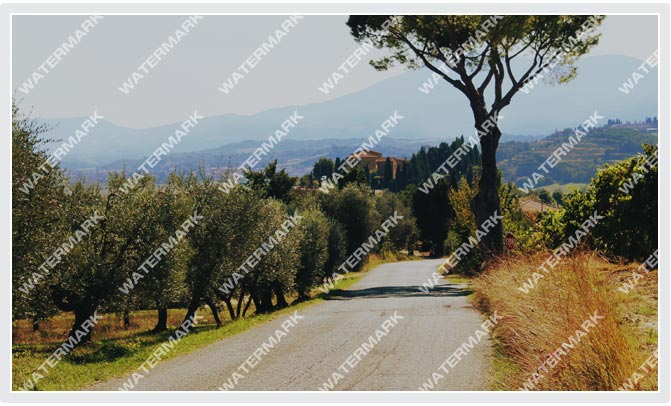
\includegraphics{ex.png}
.
.
.

\begin{enumerate}
	\item Spatial domain techniques - directly add the watermark to pixel values - exploit Human Visual System for hiding the data
	\item Transformed domain techniques - add the watermark to the coefficients of a full-frame transform (DFT, DCT, Mellin, Radon, Fresnell)
	\item Hybrid techniques
\end{enumerate}

\section{Project scope}

In the following subchapters, 

	\subsection{Goal}
	The main goal of the project is to prepare simple application with both of the algorithms implemented. Our tasks were focused on proper algorithm implementation rather than on user interface. We were trying...
	
	\subsection{Communication}
	Communication of team members took place remotely using Trello (an internet
	application for project management) and Facebook Messenger (messenger on a social
	networking site). After the division of tasks through Trello, each member could take on	a specific task and present the progress of the work and the final effects of the project stages on an ongoing basis. Important point of communication were team meetings, where we could discuss problems related to the project implementation and solve difficult tasks more efficient. The source code of the application has been managed remotely using the GitHub repository.
	
	\subsection{Features}

	
	\subsection{Requirements}
\section{Techniques and Technologies}
	
	\begin{itemize}
		\item Python 3.7
		\item NumPy
		\item scikit-image
		\item algorithms: \begin{enumerate}
			\item LSB – Least Significant Bit
			\item Patchwork techniqe
		\end{enumerate}
	\end{itemize}
	
\section{Milestone and project plan}

	\subsection{Team members}
	
	\begin{itemize}
		\item Bartosz Gardziejewski
		\item Rafał Gradkowski
		\item Łukasz Obrebski
		\item Paweł Zaborowski
	\end{itemize}

	\subsection{Project plan}
	
	Out team have splitted into topic groups:
	
	\begin{enumerate}
		\item LSB implementation
		\item Patchwork implementation
		\item Documentation work
	\end{enumerate}
	

	\subsection{Gantt Chart}
	
	\begin{itemize}
	

	\item 11.10.19 – Setup of Trello \& GitHub
	\item 17.10.19 – Project Kick OFF (first presentation)
	\item 14.11.19 – Literature analysis, working Python environment, beginnings of a documentation
	\item 28.11.19 – Implementation of embedding digital watermark in images using both algorithms
	\item 12.12.19 – Implementation of decoding digital watermark in images using both algorithms
	\item 09.01.20 – Juxtaposition and comparison of results
	\item 16.01.20 – Project closure (Final presentation, project demo, documentation)
	\end{itemize}
	
	\subsection{}
\section{Results}

	\subsection{LSB}

	    \subsection{implementation}
    	In our program the LSB algorithm is going thru the image colour by colour and pixel by pixel and checks the most significant bit of the watermark pixel, if it is 1 then it sets 1 in lest significant bit of the pixel in image, if it is 0 then it is set to 0. If the water mark is smaller then image it is looped.

    	\subsection{testing}
    	We performed test using our LSB algorithm on two pictures. The results was as follows.
    	Firs picture was python logo with resolution 225x225 it take approximately 1 second to watermark that image and the second was photo with resolution 393x206 it take approximately 1.5 second:

    	
\includegraphics[scale=3.0]{python_lsb/python_original.png}

    	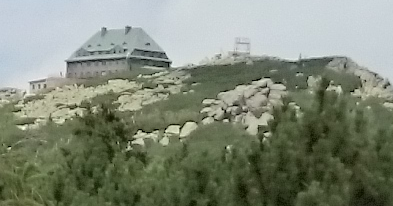
\includegraphics[scale=0.5]{photo_lsb/Photo_original.png}

        As watermark we used small python logo with resolution 64x64 and color inversion:

    	
\includegraphics[scale=1.5]{watermark.png}

        Watermarked image and the water mark extracted from it looked as expected:

    	
\includegraphics[scale=1.0]{python_lsb/watermarked_python.png}
    	
\includegraphics[scale=1.0]{python_lsb/watermark_photo.png}

    	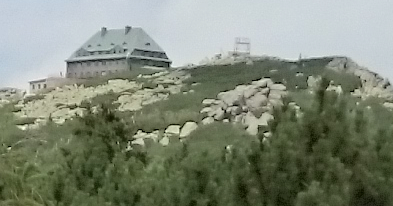
\includegraphics[scale=0.6]{photo_lsb/watermarked_photo.png}
    	
\includegraphics[scale=0.6]{photo_lsb/watermark_photo.png}

    	Next step was to transform the watermarked image and check if watermark is extractable from it. To perform transformation we used program GIMP2.0. first we try rotating image 45 degree:

    	
\includegraphics[scale=1.0]{python_lsb/watermark_python_rot45.png}
    	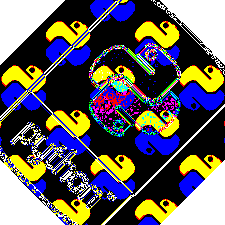
\includegraphics[scale=1.0]{python_lsb/watermark_watermark_python_rot45.png}

    	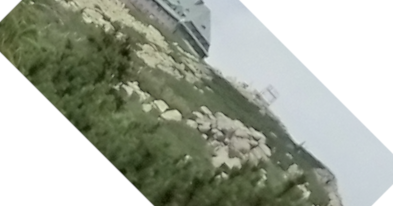
\includegraphics[scale=0.6]{photo_lsb/watermarked_photo_rot45.png}
    	
\includegraphics[scale=0.6]{photo_lsb/watermark_watermarked_photo_rot45.png}

    	Expected outcome of the rotation would be rotated wtermark, but in this case we could see distortion around edges in \textit{python} logo and absolutely unreadable watermark in \textit{photo}. It turns out that some programs have more complex rotation algorithm to maker rotated image look better. Next we try color invertion:

    	
\includegraphics[scale=1.0]{python_lsb/watermark_python_invert.png}
    	
\includegraphics[scale=1.0]{python_lsb/watermark_watermark_python_inver.png}

    	In this case as expected watermark was color inverted only. Next we try manipulate with color, and change contrast:

    	
\includegraphics[scale=1.0]{python_lsb/watermark_python_colMod.png}
    	
\includegraphics[scale=1.0]{python_lsb/watermark_watermark_python_colMod.png}

    	It Turns out that even slightly changed contrast makes watermark almost unreadable. Last transformation was more advanced one, performed on \textit{photo}.

    	Noise reduction:

    	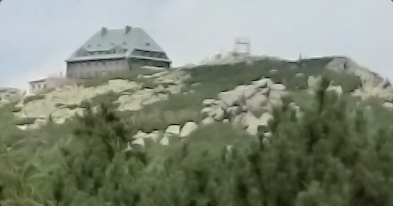
\includegraphics[scale=0.6]{photo_lsb/watermarked_photo_reduction.png}
    	
\includegraphics[scale=0.6]{photo_lsb/watermark_watermarked_photo_reduction.png}

    	Gaussian blur:

    	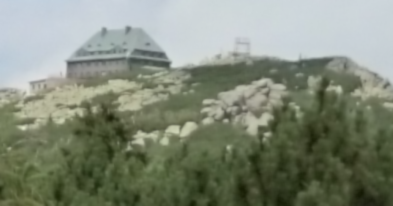
\includegraphics[scale=0.6]{photo_lsb/watermarked_photo_gaus.png}
    	
\includegraphics[scale=0.6]{photo_lsb/watermark_watermarked_photo_gaus.png}

    	They both almost completely destroyed watermark.

	\subsection{2}

	Patchwork pros and cons

	\begin{itemize}
		\item Resistance to cropping and to gamma and tone scale corrections
		\item The detector doesn’t require the original cover image to determine whether the image has been watermarked.
		\item Can be destroyed by any affine transformation, like translation, rotation or scaling
	\end{itemize}

\section{Conclusions}

	\subsection{LSB}

	LSB is fairly simple algorithm ant quite fast, unfortunately it is not very robust, simple transformation can make it "disappear", we can use for example not the least significant bit but middle one that should increase robust, although it makes watermark more visible:


	
\includegraphics[scale=1.0]{python_lsb/watermarked_python_4bit.png}


	LSB pros and cons:
	\begin{itemize}

		\item Resistance to geometric transformations, like cropping, stretching or rotating, in condition that the operation is not using more sophisticated algorithm
		\item High capacity of watermark
		\item fast and easy to implement
		\item Can be easily destroyed by distortions or gamma changes




	\end{itemize}

	

\end{document}